\documentclass[11pt]{article}

\usepackage[utf8]{inputenc}
\usepackage[T1]{fontenc}
%\RequirePackage{lmodern}	% font set: Latin Modern
\RequirePackage{charter}	% font set: Charter

\usepackage[french,english]{babel}

% Package ADDED
\usepackage{xcolor,graphics,graphicx}

% For citations
\usepackage{csquotes}

% For line spacing
\usepackage{setspace}
\linespread{1.3}

% To rotate a table or a figure
\usepackage{lscape}
% MATHS
%% The amssymb package provides various useful mathematical symbols
\usepackage{amssymb}
\usepackage{amsmath}
\usepackage{empheq}

% TAILLE de la page
\usepackage{geometry} % define page margin
\geometry{top=20mm,left=30mm,right=30mm,bottom=20mm} % margin from top, left, right and bottom

% COMPTEUR de ligne
%% The lineno packages adds line numbers. Start line numbering with
%% \begin{linenumbers}, end it with \end{linenumbers}. Or switch it on
%% for the whole article with \linenumbers after \end{frontmatter}.
\usepackage{caption}
\usepackage{lineno}
\linenumbers

% BIBLIOGRAPHIE
%\usepackage[numbers]{natbib}
\usepackage[authoryear]{natbib}
\usepackage{hyperref}

\begin{document}


% USED TO ADD "S" in front of Table, Figure, Equation
\setcounter{table}{0}
\renewcommand{\thetable}{S\arabic{table}}%
\setcounter{figure}{0}
\renewcommand{\thefigure}{S\arabic{figure}}%
\setcounter{equation}{0}
\renewcommand{\theequation}{S\arabic{equation}}%

% ------------- TITLE PAGE

\begin{center}
	\huge\textbf{
	Supporting Information 1
	}\par
\end{center}

\begin{center}
	\Large\textbf{
		Trophic transfer of anticoagulant rodenticides while managing rodent pests: the fine line between predator-prey regulation and pesticide-pest regulation
	}\par
\end{center}

\vspace{.5cm}

\begin{center}
	\large\textbf{
		Virgile Baudrot$^{1,2}$ 
		Javier Fernandez-de-Simon$^1,3$
		Michael Coeurdassier$^1$,
		Geoffroy Couval$^1,4$,
		Patrick Giraudoux$^1$,
		Xavier Lambin$^5,6$		
	}\par	
\end{center}
~\\
$^1$ Université Bourgogne Franche-Comté - UMR CNRS 6249 Laboratoire Chrono-environnement, 25030 Besançon, France\\
$^2$ BioSP, INRA, 84000 Avignon, France\\
$^3$ IREC. Instituto de Investigación en Recursos Cinegéticos\\
$^4$ FREDON Franche-Comté, Espace Valentin Est, 12, Rue de Franche-Comté - Bât E, 25480 Ecole-Valentin, France\\
$^5$ School of Biological Sciences, University of Aberdeen, Zoology Building, Tillydrone Avenue, Aberdeen AB24 2TZ, Scotland, UK\\
~\\
$^*$ Corresponding authors: virgile.baudrot@posteo.net or x.lambin@abdn.ac.uk


\newpage

% -----------------------------

\section{Model derivation}


% GRAPHIC SCHEME

\begin{figure}
	\begin{center}
		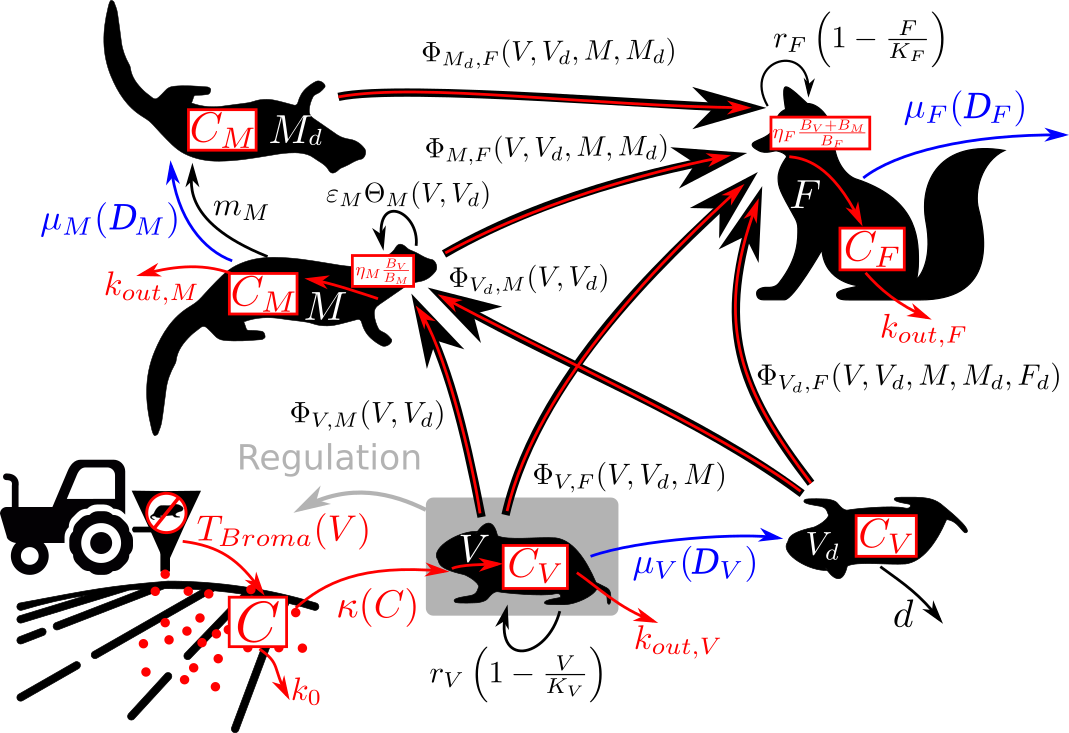
\includegraphics[width=.8\linewidth]{img/system_scheme.png}
		\caption{Dynamics of mustelids (bold grey line) and red foxes (bold black line) after 50 years of simulation (10 years of burn-in period, shaded area, and 40 years considered here for the compute of results, estimation of 
			cost functions, etc.). Letters at the top-right part of each sub-graph corresponds to the results obtained from each farmer functional response. FR (dashed line) and MR (dotted line) indicate the farmer-regulated and mustelid-regulated periods of vole population dynamics.}
		\label{fig:scheme}
	\end{center}
\end{figure}


\subsection{Dynamic of populations for the tri-trophic dynamic}
%
The population dynamics of a tri-trophic system is commonly described as follow:
\begin{equation}
\left\{
\begin{array}{l l}
\dfrac{dV}{dt} & =  r_V V \left( 1- \dfrac{V}{K_V}\right) - \Phi_{V,M}(V)M - \Phi_{V,F}(V,M)F\\[.3cm]
%
\dfrac{dM}{dt} & = \varepsilon_M \Phi_{V,M}(V)M - m_M M - \Phi_{M,F}(V,M)F\\[.3cm]
%
\dfrac{dF}{dt} & = F r_F \left( 1- \dfrac{F}{K_F}\right)
\end{array}
\right.
\label{eq:simpleSystem}
\end{equation}

As described in the manuscript, the vole population, $V$ followed a logistic growth rate, with $r_V$  the maximal reproduction rate, fixed at $r_V = \ln(2 \times 600)/365$ in [day$^{-1}$], since montane water vole populations can increase from 0  to  600 individuals ha$^{-1}$ or more in a year \citep{Giraudoux1997} resulting in the equilibrium density being fixed at $K_V = 600$ individuals. 

\subsubsection{About the logistic model}

The idea behind this parametrization is the use of a classical Malthusian equation with $r_V$ in [day$^{-1}$] and $V$ in [ind ha$^{-1}$]:

\begin{equation}
\frac{dV}{dt} = r_V V \quad \Rightarrow \quad
V(t) = V(0) \exp(r_V t) \quad \Rightarrow \quad
r_V = \ln\left( \frac{V(t)}{V(0)} \right) \times \frac{1}{t}
\end{equation}
So to have the maximal growth rate $r_V$, we need the greatest $V(t)$ (measured at 600 ind ha$^{-1}$ but supposed to be more in theoretical optimal condition) obtained in the minimum of time (less than a year). 
%
Then, to add the carrying capacity $K_V$ in [ind$^{-1}$], we use the logistic equation and assumed the carrying capacity to be the one measured in the environment:
\begin{equation}
\frac{dV}{dt} = r_V V \left( 1 - \frac{V}{K_V}\right)
\end{equation}


The estimation of $r$ using the Malthusian function and then applying the carrying capacity $K$ can be seen as non consistent because of the dependency of $r_V$ to $K_V$. 
%
For isntance, in \citet{Ginzburg1992}, the author says that going from $dV/dt = r_V V$ to $dV/dt = r_V V (1-V/K_V)$ would be correct if $r$ was independent of resource limitation $K_V$:

\textit{"Two populations  of a species live in environments  identical in all  respects, that is, they  have the same resource availability  and any  other imaginable characteristics. One of the two is subject to  higher mortality. There is no doubt  that the population growth curves in these two cases will be different. Are the final equilibrium abundances different? Most ecologists will answer that the equilibrium values should be the same and that the higher rate of reproduction just means that the population will ‘get there faster’, but reach the same level nevertheless".}


Then, \citet{Ginzburg1992} states that their is two ways to reflect the extra mortality: either assuming (a) $dV/dt = r_V V(1-V/K_V) - mV$ or (b) $dV/dt = (r_V-m_V)V(1-V/K_V)$.
%
In equation (a), the equilibirum depend on $r$: $V^* = (r_V-m_V) K_V /r_V$, so is wrong with the un-changed equilibrium assumption.
%
And re-writing (b) gives: $dV/dt = rV(1-V/K_V) - m_V V(1-V/K_V)$. Since $- m_V V(1-V/K_V)$ reflects an environmental pressure, it should not be positive when $V>K_V$. Meaning, when the population is over it’s carrying capacity, we are going to growth even faster and to infinity.
%
In the present manuscript, we made assumption (a), and we assume that $r$ is not independent of resource limitation $K_V$. It is for instance well known that vole reproduction rate is linked to the state of resource at the time of reproduction \citep{Pinot2016}.


Many authors respond to Ginzburg \citep{Olson1992, Watkinson1992, Mackenzie1992, Berryman1992} and later \citep{Gabriel2005}.  

In his response, \citet{Olson1992} says: \textit{“While the logistic model is often defined as non-mechanistic, it has the attractive feature of describing population growth with only two parameters, $K$ and $r$. $K$ is universally defined as the population-carrying capacity. However, there is much disagreement about the definition of  $r$ and this disagreement has affected conclusions derived from the use of the logistic equation.”}
%
\citet{Olson1992} suggests that the problem is the intuition assigned to the r-independence to equilibirum density $K$.
%
Again in our line, \citet{Watkinson1992} argues that \textit{"Most ecologists, he asserts, would believe that the equilibrium values of these two populations should be the same. In that case I must be one of the minority who does not believe this to be so."} 

Another answer by \citet{Berryman1992} proposed to rewrite the model in order to see the link between $r$ and $K$. The approach by \citet{Berryman1992} is interesting as it introduces a relevant effect of considering  the exploitation rate (link to the growth rate) within the carrying capacity, meaning a carrying capacity with its on dynamic (e.g., with its resilience depending on how exploitation happen), and non an extra-system static one.

\subsubsection{Predation of voles, and predator dynamics}

The vole population was preyed upon by mustelid and fox populations, denoted $M$ and $F$ respectively in \eqref{eq:simpleSystem}. The vole consumption rate at different vole densities was described by functional responses ($\Phi_{V,M}$ for mustelids, $\Phi_{V,F}$  for foxes).

\begin{equation}
\begin{array}{l l}
\Phi_{V,M}(V)M = \dfrac{a_M V}{1 + h_M a_M V} \\[.3cm]
%
\Phi_{V,F} = \dfrac{a_{VF} V}{a_{VF}V + a_{MF}F} \times \dfrac{(a_{VF}V + a_{MF} M)^2}{1 + h_F(a_{VF}V + a_{MF} M)^2}\\[.3cm]
%
\Phi_{M,F}(V,M)F = \dfrac{a_{MF}V}{a_{VF}V + a_{MF}F} \times \dfrac{(a_{VF}V + a_{MF}M)^2}{1+h_F(a_{VF}V + a_{MF}M)^2}
\end{array}
\label{eq:functionResponse}
\end{equation}


We treated small mustelids as vole specialist predators \citep{King2006}, assuming a Holling Type 2 functional response with attack rate $a_M$ in [day$^-1$] and handling time $h_M$ in [day] (equation \eqref{eq:functionResponse}). We then represented foxes feeding on voles and mustelids by a multi-species functional response derived from Holling Type 3, referring to generalist feeding behaviour \citep{Baudrot2016}. For that, we denoted $a_{VF}$ and $a_{MF}$ (both in  [day$^-1$]) the fox attack rate on voles and mustelids respectively. The parameter $h_F$ was the handling time for foxes in [day].

Consequently, the functional responses $\Phi_{X,Y}$ are all in [day$^{-1}$].  And the functions:
 
$\dfrac{dV}{dt}  =  r_V V \left( 1- \dfrac{V}{K_V}\right) - \Phi_{V,M}(V)M - \Phi_{V,F}(V,M)F$ and $\dfrac{dF}{dt} = F r_F \left( 1- \dfrac{F}{K_F}\right)$ are also consistent, all part being in [ind ha$^{-1}$ day$^{-1}$].


\subsubsection{Conversion efficiency and mortality rate in mustelid population}

The parameterization of the conversion efficiency of ingested food into new born, $\varepsilon_M$ in [n.d.] (non dimensional), and the mortality rate, $m_M$ in [day$^{-1}$], in equation \eqref{eq:simpleSystem} is not straightforward since we have to take into account the mortality rate due to starvation.
% 
In the situation of no starvation, ageing, diseases and predation of mustelids are the main reason of death. In the situation of no prey availability at initial condition, then the mortality rate of mustelids should be equal to the mortality rate without food. 
Using the simplest scheme of Dynamic Energy Budget (DEB) theory (seeFigure~\ref{fig:DEB_scheme}), the ingested food is assimilated for a part, we denote $\alpha$ and non-assimilated for another part, $(1- \alpha)$. Then, the assimilated part goes to a reserve (or directly use) in either the somatic maintenance or in the maturity maintenance (to produce reproductive tools). In DEB, a proportion $\kappa$ from the reserve is the part allocated to somatic maintenance [n.d.] and a proportion $1-\kappa$ is addressed to the maturity maintenance.


\begin{figure}
	\begin{center}
		\includegraphics[width=.5\linewidth]{img/DEB_scheme.png}
		\caption{Representation of the standard dynamic energy budget (DEB model \citep{Sousa2010}}
		\label{fig:DEB_scheme}
	\end{center}
\end{figure}

Figure~\ref{fig:DEB_scheme} represents the standard dynamic energy budget (DEB) model \citep{Sousa2010}.
%
Then, assuming the generic functional response $\Phi_{V,M}(V)$, the reproduction rate of the predator is like:
\begin{equation}
\Phi_{V,M}(V) \alpha (1 - \kappa) \varepsilon'
\end{equation}
where $\varepsilon'$ in [n.d.] is the conversion efficiency of daily assimilated food for one individual, dedicated for reproduction into newborn mustelids.

Then, $\alpha \kappa \Phi_{V,M}$ is the part allocated to somatic maintenance structure. Parameters $\alpha$ and $\kappa$ are non-dimensional [n.d.].

We can then take into account the starvation process in the mortality rate, with a food-independent mortality rate $m_{M, -\Phi}$ in [day$^{-1}$] and a part depending on food availability $m_{M, +\Phi} = \sigma \alpha \kappa \Phi_{V,M}$ in [day$^{-1}$], with $\sigma$ [n.d.] a conversion parameter.


Then, the dynamic of Mustelid given in the manuscript equation \eqref{eq:simpleSystem} could be rewritten as:
\begin{equation}
\frac{dM}{dt} = \Phi_{V,M}(V) \alpha (1 - \kappa) \varepsilon' M - \left( m_{M, -\Phi}  + \sigma \alpha \kappa \Phi_{V,M} \right) M - \Phi_{M,F}(V, M) F
\end{equation}

Which is equal to:
\begin{equation}
\frac{dM}{dt} = \left(\alpha (1 - \kappa) \varepsilon' - \sigma \alpha \kappa  \right) \Phi_{V,M}(V)  M - m_{M, -\Phi}  M  - \Phi_{M,F}(V, M) F
\end{equation}

Therefore, if we set  the food-independent mortality rate $m_M = m_{M, -\Phi}$ and the conversion efficiency of ingested food $\varepsilon_M=\alpha ((1 - \kappa) \varepsilon' - \sigma  \kappa ) $ , we get back to the equation provided in model \eqref{eq:simpleSystem} but with a clearer definition of $\varepsilon_M$.

This is why we parameterized $m_M$ in [day$^{-1}$] as the inverse of life expectancy in [day$^{-1}$], and $\varepsilon_M$ in [n.d.] as an unclear parameter derived from the null model (i.e., without AR) to reflect observed population dynamics. 

In any case, the dimension of the equation $\dfrac{dM}{dt}  = \varepsilon_M \Phi_{V,M}(V)M - m_M M - \Phi_{M,F}(V,M)F$ is well defined, since $\varepsilon_M \Phi_{V,M}(V)$ is in [day$^{-1}$].

\subsection{Dynamic of populations with AR}

After spreading by farmer, in the model AR is degraded or transferred to voles, which are exposed to the environmental contaminant mainly through ingestion of contaminated foodstuffs (i.e., trophic transfer), and AR accumulates in their tissues and is release with rate $k_{out,V}$.
%
Contaminants in an individual, the body burden, are commonly measured in concentration per mass of individual, [$\mu$g g$^{-1}$ ind$^{-1}$] (equivalent to [mg kg$^{-1}$ ind$^{-1}$] and denoted [ppm ind$^{-1}$]).
%
Predators are only exposed to contaminant through the consumption of voles, a trophic transfer, so as a function of functional response.
\\


To consider both toxicological and population dynamics within the same equation, we convert population dynamics into dynamics of their biomasses as in \citep{Huang2015EcoTox, Baudrot2018}.

We denote $V$, $V_d$ $M$, $F$ the densities of voles, dead voles, mustelids and foxes respectively ; $B_V$, $B_{V_d}$, $B_M$ and $B_F$ the mean biomass of an individual of those species in [g ind$^{-1}$], and $B_{T,V}$, $B_{T,V_d}$, $B_{T,M}$ and $B_{T,F}$ the total biomass of the population in the space unit we used, so in [g ha$^{-1}$]. In other words, $B_{T,X} = B_X \times X$. The notation $C_V$, $C_{V_d}$ $C_M$ and $C_F$ holds for the mean concentration of the contaminant in one individual, commonly called the body burden of the prey in ppm [mg kg$^{-1}$].
%
The growth function of the prey population is a function $g_X(X, C_X)$ in [day$^{-1}$] depending on the population density $X$ and the concentration of the contaminant $C_X$.
%
The dose-response curve $\mu_X(C_X)$ is defined by a log-normal cumulative distribution function as in \cite{Loos2010}.


\paragraph{Variables for the population dynamics}
%
To convert individual dynamics into biomass dynamics, we just multiplied the variable density $X$ in [ind ha$^{-1}$] with a constant $B_X$ in [g ind$^{-1}$], so that the derivative as just to be multiplied by this constant: 
%
\begin{equation}
\frac{d B_{T,X}}{dt} = \frac{d B_X X}{dt} = B_X \frac{d X}{dt} \quad \text{and so we have} \quad  \frac{d X}{dt} = \frac{1}{B_X} \times \frac{d B_{T,X}}{dt}
\label{eq:biomTOpop}
\end{equation}
%

\paragraph{Variable for the toxicant dynamics}
%
For the dynamic of toxicants, we consider an homogeneous population.

We set a new variable $w_X = C_X B_X X$ which is in [$\mu$g g$^{-1}$] $\times$ [g ind$^{-1}$] $\times$ [ind ha$^{-1}$], so that:
%
$w_X$ is in [mg ha$^{-1}$] or [mg population$^{-1}$], which is the quantity of contaminant within the population.

The dynamic of the new variable is defined with:
%
\begin{equation}
w_X = C_X B_X X = C_X B_{T,X} \quad \Rightarrow \quad \frac{dw_X}{dt} = B_X \frac{dX C_X}{dt} = B_X \left( X \frac{dC_X}{dt} + C_X \frac{dX}{dt} \right)
\end{equation}
%

As a consequence, $\dfrac{dw_X}{dt}$ is in [mg ha$^{-1}$ day$^{-1}$].


\subsubsection{Dynamic of the contaminant in the environment}

In the agro-ecotoxico-logical system, we consider an environmental concentration of contaminant denoted by $w_{ext}$ in [mg ha$^{-1}$] in order to reflect the spatially explicit spreading of AR following determined in baits per area.
%
From the Figure~\ref{fig:scheme}, we can directly provide the dynamic of this concentration:


\begin{equation}
\frac{dw_{ext}}{dt} = T_{Broma}(V) - k_0w_{ext} - \kappa(w_{ext})V B_V
\end{equation}

with $T_{Broma}(V)$ the farmer input of AR in [mg ha$^{-1}$ day$^{-1}$] depending on vole density denoted $V$ in [ind ha$^{-1}$].
%
AR concentration in baits is 50 $\mu$g g$^{-1}$ (or mg kg$^{-1}$). So when farmer spread in grasslands at quantity 7.5 to 20 kg ha$^{-1}$ day$^{-1}$, its an amount of 375 to 1000 mg ha$^{-1}$ of AR spread (i.e., mg kg$^{-1}$ $\times$ kg ha$^{-1}$ day$^{-1}$ ).


The disappearance of AR in the field, denoted $k_0$, in [day$^{-1}$], so that $k_0 w_{ext}$ is in [mg ha$^{-1}$ day$^{-1}$].
%
Such quantity, $w_{ext}$, was available in the literature, and a proportion disappeared in the environment at rate $k_0 = 0.0815$ day$^{-1}$ \citep{Sage2008}.


The function $\kappa(w_{ext})$, in [mg kg$^{-1}$ day$^{-1}$], reflects the transfer of contaminant from the environmental compartment to the vole compartment. As a consequence, the term $\kappa(w_{ext})V B_V$ is in [mg ha$^{-1}$ day$^{-1}$] ([mg kg$^{-1}$ day$^{-1}$] $\times$ [kg ha$^{-1}$]).


This rate $\kappa(w_{ext})$ was assumed to be an increasing function characterized by a maximum intake rate $M_{in}$ in [mg kg$^{-1}$ day$^{-1}$], and a half-saturation constant for ingestion $D_{in}$ in [mg ha$^{-1}$] since $w_{ext}$ is in [mg ha$^{-1}$]:

\begin{equation}
\kappa(w_{ext})= M_{in}\times \dfrac{ w_{ext}}{D_{in} + w_{ext}}
\end{equation}

So the dimension of the ingestion rate $\kappa(w_{ext})$ is the same as $M_{in}$ that is [mg kg$^{-1}$ day$^{-1}$].


\subsubsection{Dynamics of contaminant within populations}

With the previous assumption, the general model is described as follow:

\paragraph{Population dynamics}

From the equation \eqref{eq:biomTOpop}, we have: $\dfrac{d B_{T,X}}{dt} = B_X \dfrac{d X}{dt}$

\paragraph{Conversion of $w_V$ into $C_V$}

\begin{equation}
\begin{array}{c l}
\dfrac{d C_V}{dt} & = \dfrac{d w_V / B_{T,V}}{dt} = \dfrac{1}{B_{T,V}^2} \left( \dfrac{d w_V}{dt} B_{T,V} - w_V \dfrac{d B_{T,V}}{dt}\right) \\[3mm]
%
& \\[3mm]
\end{array}
\end{equation}



\begin{equation}
\left\lbrace
\begin{array}{c l}
% OUTSIDE toxic
\dfrac{dw_{ext}}{dt} & = T_{Broma}(V) - k_0w_{ext} - \kappa(w_{ext})B_{T,V} \\[3mm]
% VOLE Dynamic
\dfrac{dB_{T,V}}{dt} & =
B_{T,V} g_V(V, C_V)	- \mu_V(C_V)B_{T,V} - B_V \Phi_{V,M}(V) M - B_V \Phi_{V,F}(V,M) F\\[3mm]
% VOLE toxic
\dfrac{dw_{V}}{dt} & = \kappa(w_{ext}) B_{T,V} - k_{out, V} w_V - w_V \mu(C_V) - C_V B_V \Phi_{V,M}(V)M + \gamma_V w_V g_V(V, C_V)\\[3mm]
%
% DEAD VOLE Dynamic
\dfrac{dB_{T,V_d}}{dt} & = \mu_V(C_V)B_{T,V}\\[3mm]
% DEAD VOLE toxic
\dfrac{dw_{V_d}}{dt} & = \dfrac{dw_{V}}{dt}\\[3mm]
%
% MUSTELID dynamic
\dfrac{dB_{T,M}}{dt} & =
B_{T,M} (\varepsilon_MB_V  \Phi_{V,M}(V)M - m_M - \mu_M(C_M) ) - B_M \Phi_{M,F}(V, M) F\\[3mm]
% MUSTELID toxic
\dfrac{dw_{M}}{dt} & = - k_{out, M} w_M - w_M (m_M + \mu(C_M)) + \eta_M C_M B_M \Phi_{V,M}(V)M - \\[3mm]
& C_M B_M \Phi_{M,F}(V,M)F + \gamma_M w_M g_M(M, C_V)\\[3mm]
%
% FOX dynamic
\dfrac{dB_{T,F}}{dt} & =
B_{T,F} g_F(F, C_F)	- \mu_F(C_F) \\[3mm]
% FOX toxic
\dfrac{dw_{F}}{dt} & = - k_{out, F} w_F - w_F \mu(C_F) + \eta_F C_M B_M \Phi_{M,V} F  + \eta_F C_V B_V \Phi_{V,V} F + \gamma_F w_F g_F(F, C_F)\\[3mm]
\end{array}
\right.
\end{equation}


%

Thus, it is straightforward to express the dynamics as:


\begin{equation}
\left\lbrace
\begin{array}{c l}
% VOLE Dynamic
\dfrac{dV}{dt} & =
\overbrace{	r_V V (1-V/K_V)		}^{\text{growth rate}} -
\overbrace{	\mu_V(C_V)V	}^{\text{poisoning}} -
\overbrace{	\Phi_{V,M}(V,V_d)M - \Phi_{V,F}(V,V_d,M)F	}^{\text{predation}}\\[3mm]
%
% DEAD VOLE Dynamic
\dfrac{dV_d}{dt} & =
\overbrace{ \mu_V(C_V)V }^{\text{new dead voles}} -
\overbrace{	\Phi_{V_d,M}(V,V_d)M - \Phi_{V_d,F}(V,V_d,M)F	}^{\text{predation}}-
\overbrace{d V_d}^{\text{degradation}}
\\[3mm]
%
% MUSTELIDS Dynamic
\dfrac{dM}{dt} & =
\overbrace{	(\varepsilon_M\Theta_M(V,V_d)-m_M) M	}^{\text{growth rate}} - 
\overbrace{\mu_M(C_M)M	}^{\text{poisoning}} -
\overbrace{\Phi_{M,F}(V,V_d,M)F }^{\text{predation}} \\[3mm]
%
% F0X Dynamic
\dfrac{dF}{dt} & =
\overbrace{	r_F F (1-F/K_F)	}^{\text{growth rate}} -
\overbrace{\mu_F(C_F)F	}^{\text{poisoning}}  \\
%
%
% Toxicological dynamics
\dfrac{dC}{d t}  & = 
\overbrace{T_{Broma}(V)}^{\text{treatment}} - 
\overbrace{k_0 C}^{\text{degradation}} -
\overbrace{\kappa(C)}^{\text{consumption}} \\[3mm]
%
% Toxico-kinetics in Voles
\dfrac{dC_V}{dt} &= 
\overbrace{\kappa(C)}^{\text{intake}} - 
\overbrace{C_V\left(k_{out,V} + r_V \left(1 - \dfrac{V}{K_V}\right)\right)}^{\text{excretion}}\\[3mm]
%
% Toxico-kinetics in Mustelids
\dfrac{dC_M}{d t} & =
\overbrace{\eta_M \dfrac{B_V}{B_M} (\Phi_{V,M}(V,V_d,M)+\Phi_{V_d,M}(V,V_d,M)) C_V}^{\text{intake}} -
\overbrace{C_M\left(k_{out,M} + \varepsilon_M \Phi_{V,M}(V,V_d,M) \right)}^{\text{excretion}} \\[3mm]
%
% Toxico-kinetics in Foxes
\dfrac{dC_F}{d t} &=
\overbrace{ \eta_F \dfrac{B_V}{B_F} \left( (\Phi_{V,M}(V,V_d,M)+\Phi_{V_d,M}(V,V_d,M)) C_V + \Phi_{M,F}(V,V_d,M) C_M \right)}^{\text{intake}} - \\[3mm]
&
\overbrace{k_{out,F} + r_F \left(1 - \dfrac{F}{K_F}\right) }^{\text{excretion}} 
\end{array}
\right.
\label{eq:Sys_complet}
\end{equation}



% BIBLIOGRAPHY
% \section*{References}

%\bibliographystyle{elsarticle-harv}
\bibliographystyle{plainnat}
%\bibliographystyle{unsrt}
\bibliography{trophToxNTO.bib}



\end{document}
